\subsection{Media access and fault tolerance layer}
\label{sec:bus:design:layer2}

The second layer of our protocol can be seen as a composition of two internal layers, 
namely the media access sublayer controlling the basic bus access as depicted in section 
\ref{sec:bus:basicaccess} \nameref{sec:bus:basicaccess} and the state machine defining 
the communication process and the fault tolerant sublayer providing basic fault 
tolerant mechanisms like the starvation handling (see section \ref{sec:bus:ftnsh}).\\

% These two sublayers and their interactions are described in the sections 
% \ref{sec:bus:design:layer2:mac} \nameref{sec:bus:design:layer2:mac} and 
% \ref{sec:bus:design:layer2:ft} \nameref{sec:bus:design:layer2:ft} in detail. 
In the following section we describe the general workflow of the MAC \& FT layer.

\subsubsection{General workflow}
To describe the general workflow of the MAC \& FT layer we examine how messages are sent and received. 
See figure \ref{fig:bus:design:layer2:statemachine} for a flow chart of the bus protocol.\\

\paragraph{Transmission of messages}
When a higher layer (including the application) wants to send a message it adds the message to the \textit{Send Msg Queue} which is provided
by a ring buffer holding all the messages payloads and the messages types. The highest prior message is stored in the protocols state machine, waiting for the bus to be free.\\

When the bus seems to be free, e.g. the transmission of a previous message has completed, the protocol tries to arbitrate the bus via the message type delivered through the message description held in the queue.\\

If the arbitration was successful the rest of the message is transmitted and the next message from the queue is fetched into the protocols finite state machine. Otherwise the message is kept in the finite state machine of the protocol and retransmitted when the bus is free again.
Whenever there was a transmission attempt whether successful or not a callback routine is fired propagating the current status of the protocol to higher level layers or to the flags and registers separating the application from the communication network interface.\\

\paragraph{Reception of messages}
When the USART reports the reception of data the protocol changes in a receiving state in which it is not allowed to transmit data.
Whenever data is receipt by the USART the fault tolerant non starvation protocol resets the timer providing basic error detection in the time domain.\\

When the timer triggers an interrupt the node knows that the transmitting node has timed out and that it can change in an idle state or transmit its own messages.\\

When a message is completely received its integrity is checked trough the CRC checksum and the message is added to the \textit{Receive Message Queue} and a \textit{Receive Callback} is triggered, informing higher level layers of the data receipt and updating the registers and flags of the CNI mapping.

%\subsubsection{Mac \& FT layer interface}
\label{sec:bus:design:layer2:interface}

The Mac \& FT layer  provides its interfaces in such a way as it takes only data via methods and returns data only via callback routines (which can be seen as events).\\

The methods provided by the interface are

\begin{enumerate}
 \item \textbf{initialize: } initializes the layer and triggers the initialization of the sublayers it uses.
 \item \textbf{writeMessage: } takes an arbitrary message payload and the payloads size in bytes, appends it to the \textit{send queue} and triggers the transmission of the next message in the queue.
 \item \textbf{writeMessageImmediate: } takes an arbitrary message payload and the payloads size in bytes, inserts it at the next position to be read in the \textit{send queue} and triggers the transmission of the next message in the queue.
\end{enumerate}

and the events provided by the interface are

\begin{enumerate}
 \item \textbf{messageReceivedCallback}
 \item \textbf{messageTransmittedCallback}
 \item \textbf{queueOverflowCallback}
\end{enumerate}










The workflow of the layers statemachine is depicted in figure \ref{fig:bus:design:layer2:statemachine} and starts in the state \textit{STARTUP}, in which a state ``synchronzies'' to the bus.

After this process the statemachine changes to state \textit{IDLE}.
When a message is appended to the queue in state \textit{IDLE} the CRC of the message is calculated and the transmission is started (\textit{SND\_ARBITRATION}) by trying the bus arbitration.\\

After the arbitration was done successfully the remaining message is transmitted in the state \textit{SND\_DATA/CRC} and the event \textit{messageTransmittedCallback} is triggered, otherwise the meanwhile received/sent data is handed out to the receive procedure and the state \textit{RCV\_ARBITRATION} is reached in which messages sent by other communication partners are received.\\

When an arbitration of another node is detected in state \textit{IDLE} the statemachine switches to state \textit{RCV\_ARBITRATION} and the receiving procedure can be done.\\

Whenever a message is successfully received the message is appended to the \textit{recv queue} and the \textit{messageReceivedCallback} event is triggered notifying higher layers of the message arrival.\\

In case the \textit{send queue} or the \textit{recv queue} overflows and data is lost the event \textit{queueOverflowCallback} is triggered to notify higher layers.\\

\begin{figure}[H]
\centering
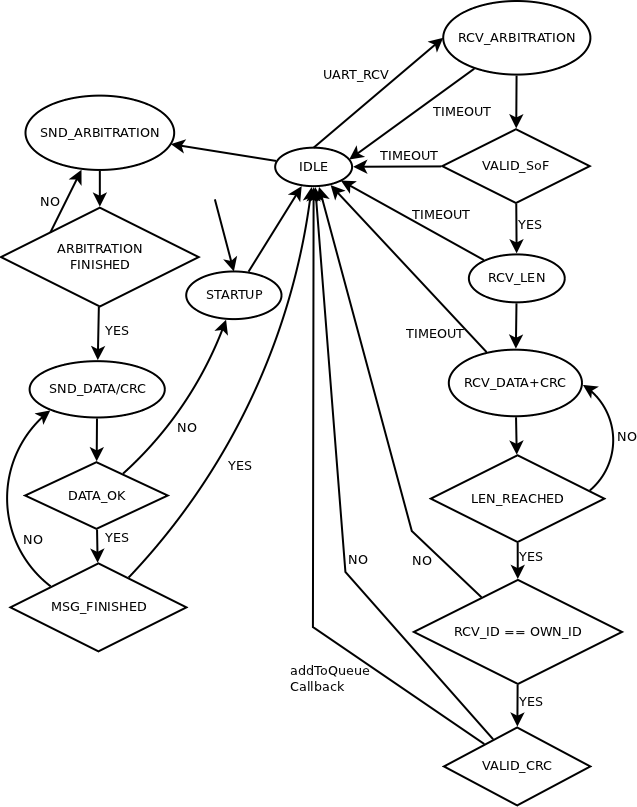
\includegraphics[width=0.8\textwidth]{../images/layer2_state_machine.png}
\caption{Layer2 state machine}
\label{fig:bus:design:layer2:statemachine}
\end{figure}